\chapter{รายละเอียดการปฏิบัติงาน}
\label{chapter:working-detail}

เริ่มสหกิจศึกษาโดยปฏิบัติงานที่ บริษัท วงใน มีเดีย จำกัด (สำนักงานใหญ่) ตั้งแต่วันที่ 4 มิถุนายน พ.ศ.2562 จนถึง 29 พฤศจิกายน พ.ศ.2562 รวมเป็นระยะเวลาประมาณ 6 เดือน โดยในการปฏิบัติงานต่าง ๆ ในช่วงสหกิจศึกษา มีรายละเอียดดังต่อไป

\section{ตำแหน่ง/หน้าที่ของงานที่ได้รับมอบหมาย}
ปฏิบัติงานด้วยตำแหน่ง Software Engineer (Backend) ทำหน้าที่รับผิดชอบในการพัฒนาและดูแลเซิร์ฟเวอร์ของเว็บไซต์ wongnai.com เพื่อให้ผู้ใช้งานทุกแพลตฟอร์มทั้งเว็บไซต์และ แอปพลิเคชันมือถือสามารถทำงานร่วมกันได้อย่างมีประสิทธิภาพ, ควบคุมคุณภาพของโค้ดให้มีคุณภาพที่ดี, ทำงานได้ถูกต้อง, ทดสอบและดูแลได้ง่าย, มีความยืดหยุ่นพร้อมรับการเปลี่ยนแปลงในอนาคต

\section{รายละเอียดของโครงงานที่รับผิดชอบ}
โครงงานที่รับผิดชอบคือ ระบบจัดการโฆษณาแบบจำกัดจำนวนการคลิกและการแสดงโฆษณา เป็นระบบที่พัฒนาขึ้นมาใหม่ต่อจากระบบเดิม ซึ่งจะทำให้ลูกค้าสามารถลงโฆษณากับทาง Wongnai แบบจำกัดจำนวนการแสดงผลและการคลิกได้ อีกทั้งยังสามารถส่งอีเมลรายงานผลการโฆษณากลับไปยังลูกค้าทุก ๆ สัปดาห์โดยอัตโนมัติอีกด้วย เพื่อให้สามารถส่งมอบงานได้เร็วที่สุดและระบบทำงานได้จริง จึงได้พัฒนาฟังก์ชันหลัก 2 ประการ ได้แก่
\begin{itemize}
	\item จำกัดการแสดงโฆษณาของร้านด้วยจำนวนการคลิกโฆษณาได้
	\item สามารถส่งอีเมลรายงานผลการโฆษณากลับไปยังลูกค้าโดยอัตโนมัติได้
\end{itemize}

\section{แนวคิดและทฤษฎีที่เกี่ยวข้อง}
\begin{enumerate}
	\item Cost Per Click (CPC)
	
	CPC เป็นรูปแบบการโฆษณาผ่านทางอินเตอร์เน็ตอย่างหนึ่ง เพื่อเป็นการเพิ่มยอดผู้ชมของเว็บไซต์  โดยจะเสียค่าใช้จ่ายก็ต่อเมื่อมีการคลิกไปยังโฆษณาที่แสดงไว้ ~\cite{cpc}
	
	\item ไมโครเซอร์วิส
	
	ไมโครเซอร์วิสเป็นสถาปัตยกรรมที่เกิดขึ้นจากสถาปัตยกรรมเชิงบริการ (Service-Oriented Architecture) โดยจะแยกแอปพลิเคชันออกเป็นเซอร์วิสขนาดเล็ก มีความสามารถในการจัดการด้วยตัวเอง, มีความเป็นอิสระต่อกัน และมีความยิดหยุ่นพร้อมต่อการเปลี่ยนแปลง ~\cite{microservices} โดยแต่ละเซอร์วิสนั้นจะมีฐานข้อมูลเป็นของตัวเองหรือจะไม่มีก็ได้ แต่จะไม่ใช้ฐานข้อมูลร่วมกัน และเซอร์วิสสามารถเรียกใช้งานอีกเซอร์วิสหนึ่งได้ แต่อีกเซอร์วิสหนึ่งจะไม่ไปเรียกใช้งานอีกเซอร์วิส เช่น เซอร์วิส 3 เรียกใช้งานเซอร์วิส 2 แต่เซอร์วิส 2 จะไม่ไปเรียกใช้งานเซอร์วิส 3 ทั้งนี้เพื่อไม่ให้เป็นการทำให้เซอร์วิส 2 เซอร์วิสถูกผูกมัดซึ่งกัน
	\begin{figure}[!h]
		\centering
		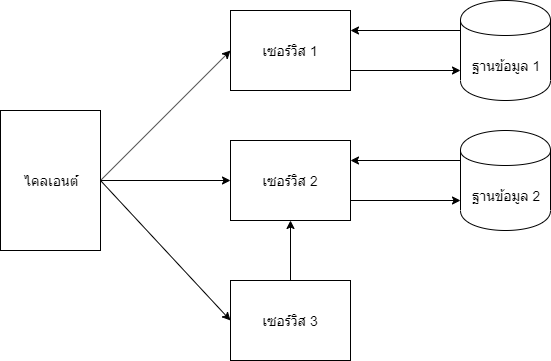
\includegraphics[width=0.8\textwidth]{microservices}  
		\caption{แผนผังแสดงตัวอย่างการออกแบบระบบโดยใช้สถาปัตยกรรมไมโครเซอร์วิส}
		\label{Fig:microservices}
	\end{figure}

	\item REST (Representational state transfer)

	REST เป็นสถาปัตยกรรมซอฟต์แวร์อย่างหนึ่งในการสร้างเว็บเซอร์วิส ทำให้แต่ละเซอร์วิสสามารถทำงานร่วมกันได้ผ่านเครือข่ายอินเตอร์เน็ต มักจะใช้ HTTP (Hypertext Transfer Protocol) เป็นโปรโตคอลในการสื่อสาร โดย HTTP นั้นเป็นโปรโตคอลแบบ Stateless ทำให้มีสมรรถภาพสูง, มีความน่าเชื่อถือ และมีความสามารถในการนำกลับไปใช้ใหม่ได้โดยไม่กระทบกับระบบส่วนอื่นแม้ว่าระบบกำลังทำงานอยู่ก็ตาม ~\cite{rest}
	
	\item HTTP (Hypertext Transfer Protocol)
	
	HTTP เป็นโปรโตคอลในการส่งข้อมูลบนเว็บ เป็นโปรโตคอลแบบไคลเอนต์-เซิร์ฟเวอร์ โดยไคลเอนต์จะส่งคำร้องขอข้อมูลไปยังเซิร์ฟเวอร์ จากนั้นเซิร์ฟเวอร์ก็จะส่งคำตอบกลับมาที่ไคลเอนต์ ~\cite{http}

	\begin{figure}[!h]
		\centering
		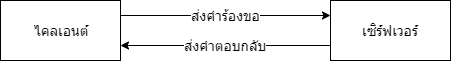
\includegraphics[width=0.8\textwidth]{http}  
		\caption{แผนผังแสดงตัวอย่างการสื่อสารด้วยโปรโตคอล HTTP}
		\label{Fig:http}
	\end{figure}

	\item Repository Pattern
	
	Repository Pattern เป็นรูปแบบหนึ่งในการออกแบบเซอร์วิส โดย Repository เป็นคลาสที่ห่อหุ้มลอจิกต่าง ๆ ที่เอาไว้เข้าถึงแหล่งข้อมูล ทำให้สามารถเข้าถึงข้อมูลเพียงแค่ใช้ฟังก์ชัน, ง่ายต่อการดูแลรักษา และแยกส่วนการทำงานระหว่างเทคโนโลยีที่เอาไว้เข้าถึงแหล่งข้อมูลออกจากโดเมนเลเยอร์ของโมเดล ~\cite{repository} ยกตัวอย่างเช่น มีคลาสของออบเจ็กต์ชื่อว่า Product และออบเจ็กต์ถูกเก็บอยู่ในฐานข้อมูล เมื่อมีลอจิกทางธุรกิจใดก็ตามที่ต้องการค้นหา Product ตามชื่อที่ต้องการ เราสามารถใช้เมธอด findByName ของคลาส ProductRepository เพื่อทำการค้นคืนข้อมูลออบเจ็กต์ Product ที่เราต้องการได้ทันที
	
	\begin{figure}[!h]
		\centering
		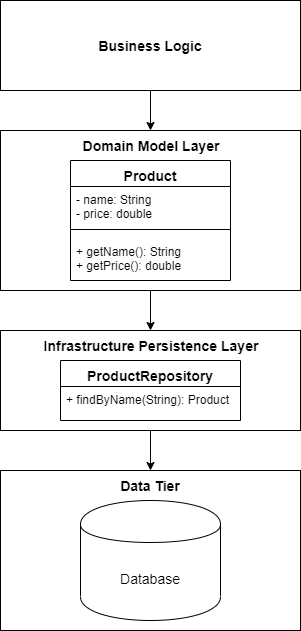
\includegraphics[width=0.5\textwidth]{repository}  
		\caption{แผนผังแสดงตัวอย่างของ Repository Pattern}
		\label{Fig:repository}
	\end{figure}
	
	\item Object-Relational Mapper (ORM)
	
	Object-Relational Mapper เป็นการแปลงออบเจ็กต์ที่เกิดขึ้นจากแนวคิดการเขียนโปรแกรมเชิงวัตถุ (Object-Oriented Programing) ให้สามารถใช้งานกับฐานข้อมูลประเภท Relational ได้ ~\cite{orm} ยกตัวอย่างเช่น คลาส Product มีคุณลักษณะต่าง ๆ ได้แก่ id, name และ price เมื่อนำ ORM มาใช้เพื่อแปลงออบเจ็กต์ของคลาสนี้ไปอยู่ในรูปของ Relation ก็จะได้ Relation ที่มีโครงสร้างดังรูปที่ 2.4
	
	\begin{figure}[!h]
		\centering
		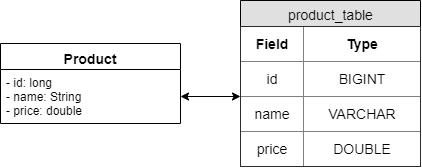
\includegraphics[width=0.8\textwidth]{orm}  
		\caption{ตัวอย่างของการแปลงออบเจ็กต์ของคลาสไปเป็น Relation ด้วย Object-Relational Mapper}
		\label{Fig:orm}
	\end{figure}
	
	\item คอนเทนเนอร์
	
	คอนเทนเนอร์เป็นหน่วยของซอฟต์แวร์ที่ทำการบรรจุโค้ดและส่วนอื่น ๆ ที่เกี่ยวข้องเอาไว้ทั้งหมดเพื่อให้สามารถรันได้ทันทีในสภาพแวดล้อมใดก็ได้ มีความเป็นมาตรฐาน และประหยัดทรัพยากร เนื่องจากในการรันหลาย ๆ แอปพลิเคชันที่เป็นคอนเทนเนอร์พร้อมกันจะใช้แค่ระบบปฏิบัติการเดียว
	
	\begin{figure}[!h]
		\centering
		\subfigure[]{
			\label{Fig:infra:container}
			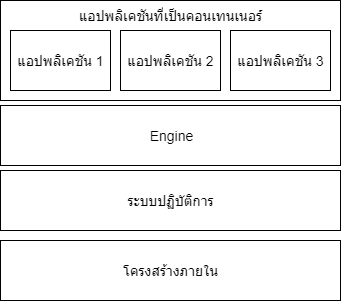
\includegraphics[width=0.45\textwidth]{container-infra}  
		}
		\subfigure[]{
			\label{Fig:infra:vm}
			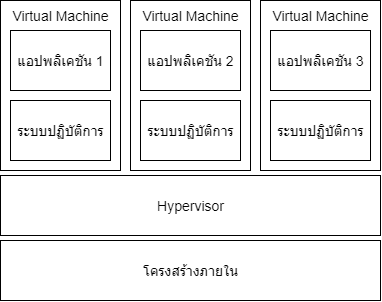
\includegraphics[width=0.5\textwidth]{vm-infra}  
		}
		\caption{แผนผังแสดงโครงสร้างเบื้องต้นภายในเซิร์ฟเวอร์เมื่อทำการใช้งาน Docker (ก) กับ Virtual Machine (ข)}
		\label{Fig:infra}
	\end{figure}

	จากรูป 2.5 (ข) แสดงให้เห็นว่า Virtual Machine ทั้งหมดจำเป็นต้องมีระบบปฏิบัติการเป็นของตนเอง ทำให้สิ้นเปลืองทรัพยากรของเซิร์ฟเวอร์โดยไม่จำเป็น แต่คอนเทนเนอร์สามารถรันร่วมกันได้โดยใช้ระบบปฏิบัติการร่วมกัน และมี Engine เป็นตัวจัดการการทำงานของแต่ละคอนเทนเนอร์ ทำให้ประหยัดทรัพยากรของเซิร์ฟเวอร์ และประหยัดค่าใช้จ่ายในเรื่องลิขสิทธิ์ของระบบปฏิบัติการที่ใช้รันเซิร์ฟเวอร์ ~\cite{docker}
	
	\item Orchestration
	
	Orchestration เป็นตัวจัดการระบบคอมพิวเตอร์และซอฟต์แวร์ รวมไปการตั้งค่าต่าง ๆ และการประสานงานกับซอฟต์แวร์อื่น ๆ โดยอัตโนมัติ ~\cite{orchestration}
	
\end{enumerate}

\section{เครื่องมือและเทคโนโลยีที่ใช้ในการปฏิบัติงาน}
\begin{enumerate}
	\item IntelliJ IDEA
	
	IntelliJ IDEA เป็น Integrate Development Environment (IDE) สำหรับใช้ในการพัฒนาซอฟต์แวร์ที่ใช้ Java Virtual Machine (JVM) โดยเฉพาะ มีระบบแนะนำการเขียนโค้ดกับระบบเติมคำอัตโนมัติที่ทำให้การเขียนโค้ดเป็นไปอย่างราบรื่นและรวดเร็ว ~\cite{intellij}
	
	\begin{figure}[!h]
		\centering
		\subfigure[]{
			\label{Fig:intellij:suggestion}
			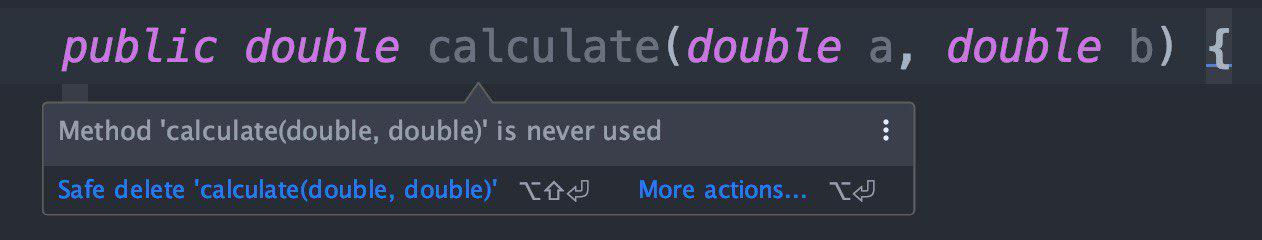
\includegraphics[width=0.8\textwidth]{suggestion}  
		}
		\subfigure[]{
			\label{Fig:intellij:auto-completion}
			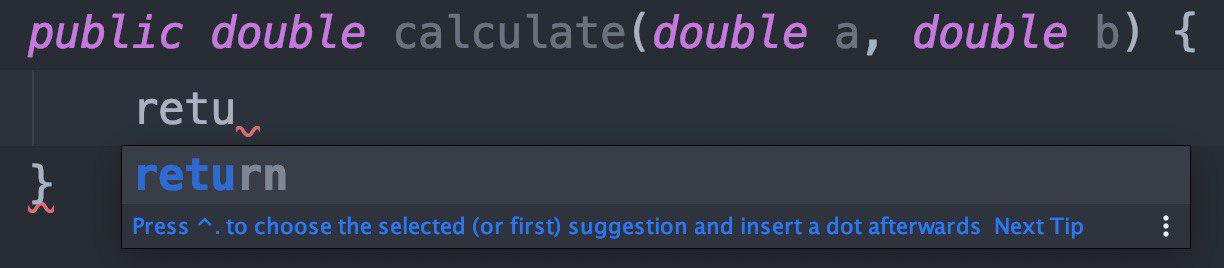
\includegraphics[width=0.8\textwidth]{auto-completion}  
		}
		\caption{ระบบแนะนำการเขียนโค้ด (ก) กับระบบเติมคำอัตโนมัติ (ข) ของ IntelliJ IDEA}
		\label{Fig:intellij}
	\end{figure}
	
	\item Visual Studio Code
	
	Visual Studio Code เป็น Text Editor ที่รองรับได้หลากหลายภาษา มีระบบไฮไลท์ Syntax ในการตรวจสอบ Syntax ของโค้ด และสามารถติดตั้งส่วนขยายต่าง ๆ เพิ่มเติมได้ตามความเหมาะสมในการทำงาน ~\cite{vscode}
	
	\item Java
	
	Java เป็นภาษาคอมพิวเตอร์ประเภท Object-Oriented เมื่อคอมไพล์แล้วจะได้ bytecode โดยเราสามารถนำ bytecode นี้ ไปใช้งานบนคอมพิวเตอร์เครื่องไหนก็ได้ที่มี Java Virtual Machine (JVM) ~\cite{java}
	
	\item Spring Boot
	
	Spring Boot คือ เฟรมเวิร์คสำหรับพัฒนา REST API, Websocket, Web และอื่น ๆ ของภาษาที่ใช้ Java Virtual Machine (JVM) ~\cite{spring}
	
	\item Hibernate ORM
	
	Hiberate ORM คือ เฟรมเวิร์ค Object Relation Mapping ที่จะแปลงออบเจกต์ให้ใช้งานกับฐานข้อมูลประเภท Relational ได้โดยผ่านทาง JDBC (Java Database Connectivity) ซึ่งเป็น API สำหรับภาษา Java เพื่อให้สามารถเข้าถึงฐานข้อมูลได้ ~\cite{hibernate}

	\item Maven
	
	Maven คือ ซอฟแวร์จัดการโปรเจค ช่วยลดขั้นตอนในการ Build ซอฟต์แวร์, ทำให้การ Build ซอฟต์แวร์เป็นมีระเบียบมากขึ้นโดยใช้ project object model (POM) ซึ่งเป็นไฟล์ .xml และช่วยจัดการ Dependencies ที่เกี่ยวข้องกับ Project ~\cite{maven}
	
	\begin{figure}[!h]
		\centering
		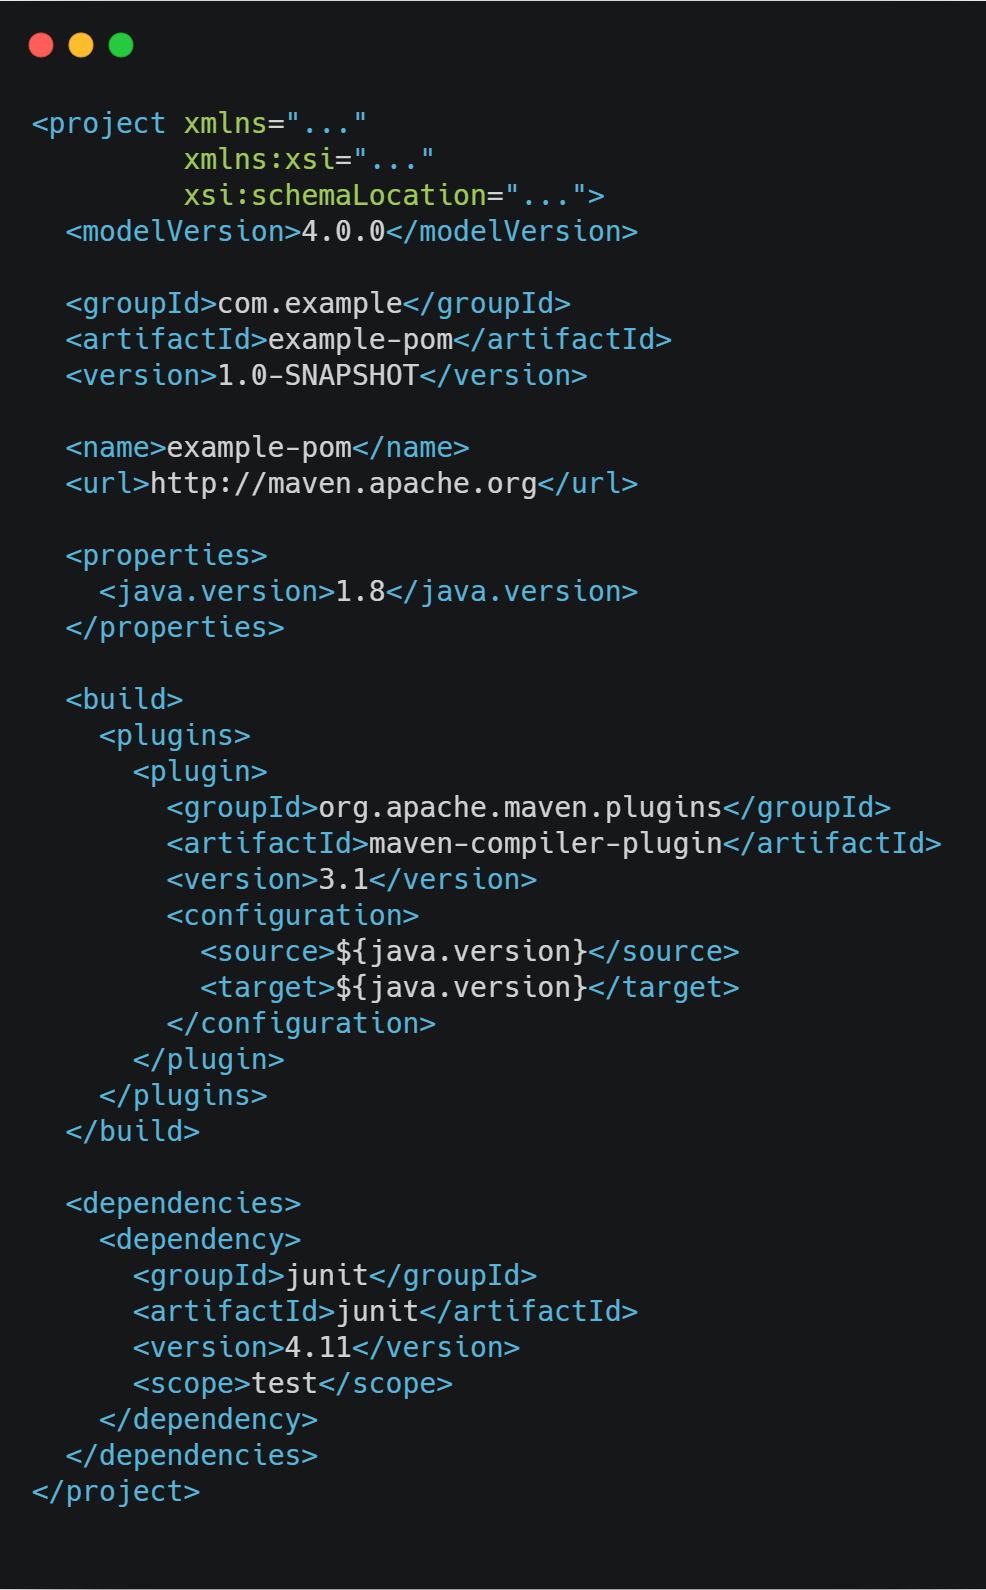
\includegraphics[width=0.7\textwidth]{pom}  
		\caption{ตัวอย่างไฟล์ pom.xml ของ Maven}
		\label{Fig:pom}
	\end{figure}
	
	\item Python
	
	Python เป็นภาษาคอมพิวเตอร์ระดับสูงที่ใช้ Python Interpreter มีจุดเด่นที่สามารถอ่านและทำความเข้าใจโค้ดได้ง่าย โดย Python Interpreter นั้น สามารถติดตั้งได้ในหลากหลายระบบปฏิบัติการ ~\cite{python}
		
	\item MySQL
	
	MySQL เป็นตัวจัดการฐานข้อมูลแบบ Relational ที่เป็น Open source ~\cite{mysql}

	\item Sequel Pro
	
	Sequel Pro เป็นแอปพลิเคชันสำหรับจัดการฐานข้อมูล MySQL ~\cite{sequelpro}
	
	\item Google BigQuery
	
	Google BigQuery เป็นบริการคลังข้อมูลบน Cloud ที่ให้บริการโดย Google และสามารถใช้ SQL เพื่อใช้งาน Google BigQuery ได้ ~\cite{bigquery}
	
	\item Git
	
	Git คือ Version Control ที่สามารถติดตามและควบคุมการเปลี่ยนแปลงของโค้ดได้ เพื่อให้ Software Engineer คนอื่น ๆ สามารถทำงานร่วมกันได้อย่างมีประสิทธิภาพ ~\cite{git}
	
	\item GitKraken
	
	GitKraken เป็น Git GUI Client ที่ทำให้สามารถใช้งาน Git ได้อย่างสะดวกสบาย ~\cite{gitkraken}

	\item Postman
	
	Postman เป็นแอปพลิเคชันสำหรับสร้างคำร้องขอไปยังเซิร์ฟเวอร์ เช่น REST, SOAP, GraphQL เพื่อทดสอบการทำงาน API (Application Programming Interface) ของเซิร์ฟเวอร์ และสามารถตรวจสอบคำตอบกลับที่ส่งกลับมาได้ ~\cite{postman}
	
	\item Docker
	
	Docker คือ คอนเทนเนอร์ Engine สำหรับสร้างและจัดการคอนเทนเนอร์ของซอฟต์แวร์ ทำให้ซอฟต์แวร์สามารถนำไปใช้งานในสภาพแวดล้อมไหนก็ได้ โดยเราสามารถเขียน Dockerfile เพื่อสร้างอิมเมจของคอนเทนเนอร์ได้ หรือจะใช้อิมเมจสาธารณะจาก Docker Hub ก็ได้ ~\cite{docker}
	
	\begin{figure}[!h]
		\centering
		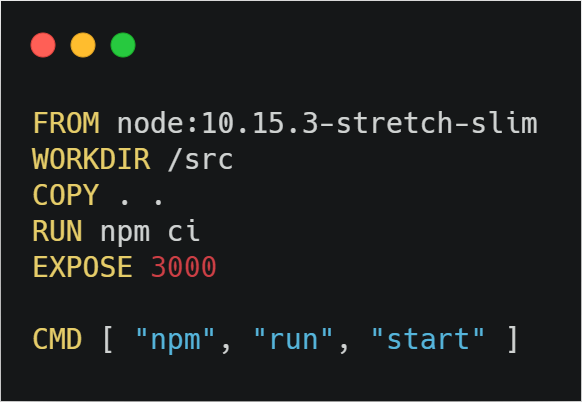
\includegraphics[width=0.5\textwidth]{dockerfile}  
		\caption{ตัวอย่างไฟล์ Dockerfile ในการตั้งค่าเพื่อการสร้างอิมเมจของคอนเทนเนอร์}
		\label{Fig:dockerfile}
	\end{figure}
	
	\item Kubernetes	
	
	Kubernetes คือ Orchestration ของกลุ่มคอนเทนเนอร์และกลุ่มเซิร์ฟเวอร์ มีความสามารถในการจัดการคอนเทนเนอร์ให้สามารถทำงานได้อย่างต่อเนื่อง มีช่วงเวลาหยุดทำงานเป็นศูนย์ 	 ~\cite{kubernetes} โดย Kubernetes ยังมีฟังก์ชันอำนวยความสะดวกอื่น ๆ เช่น
	\begin{itemize}
		\item กระจายโหลดที่เข้ามายังคอนเทนเนอร์ เพื่อให้สามารถทำงานได้อย่างมีเสถียรภาพ
		\item ตั้งค่าให้ Kubernetes จัดสรรทรัพยากรต่าง ๆ กับคอนเทนเนอร์ได้ เช่น หน่วยความจำ และหน่วยประมวลผล เป็นต้น โดย Kubernetes จะจัดการเพื่อให้คอนเทนเนอร์ทำงานได้เต็มประสิทธิภาพตามทรัพยากรที่กำหนดไว้
		\item เริ่มต้นการทำงานคอนเทนเนอร์ที่หยุดทำงานให้ใหม่ สับเปลี่ยนคอนเทนเนอร์ ลบคอนเทนเนอร์ที่ไม่มีการตอบสนอง และจะไม่อนุญาตให้ใช้งานคอนเทนเนอร์ ถ้าไม่อยู่ในสถานะพร้อมใช้งานจริง ๆ
		\item เก็บข้อมูลความลับต่าง ๆ ได้ โดยสามารถ Deploy และอัปเดตข้อมูลลับและการตั้งค่า โดยที่ไม่ต้อง Build คอนเทนเนอร์ใหม่
	\end{itemize}
	ในการตั้งค่าต่าง ๆ ให้กับ Kubernetes จะต้องเขียนไฟล์ .yaml หรือ .yml ซึ่งเป็นภาษามาตรฐานของชุดข้อมูลสำหรับทุกภาษาโปรแกรมมิ่ง ~\cite{yaml}
	
	\begin{figure}[!h]
		\centering
		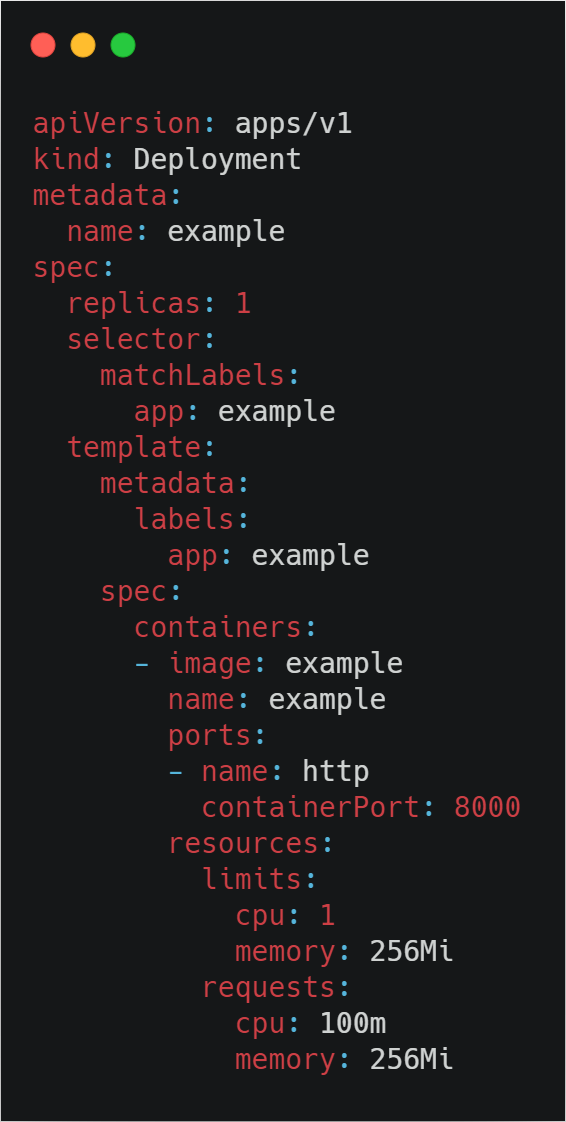
\includegraphics[width=0.4\textwidth]{k8sconfig}  
		\caption{ตัวอย่างไฟล์ .yml หรือ .yaml ในการตั้งค่าให้กับ Kubernetes}
		\label{Fig:cicdyaml}
	\end{figure}
	
	\item Gitlab CI/CD
	
	Gitlab CI/CD คือ เครื่องมือในการ Build ซอฟต์แวร์และ Deploy โดยอัตโนมัติ โดยเราสามารถตั้งค่าการทำงานของ Gitlab CI/CD ได้จากไฟล์ .gitlab-ci.yml ~\cite{gitlabcicd}
	
	\begin{figure}[!h]
		\centering
		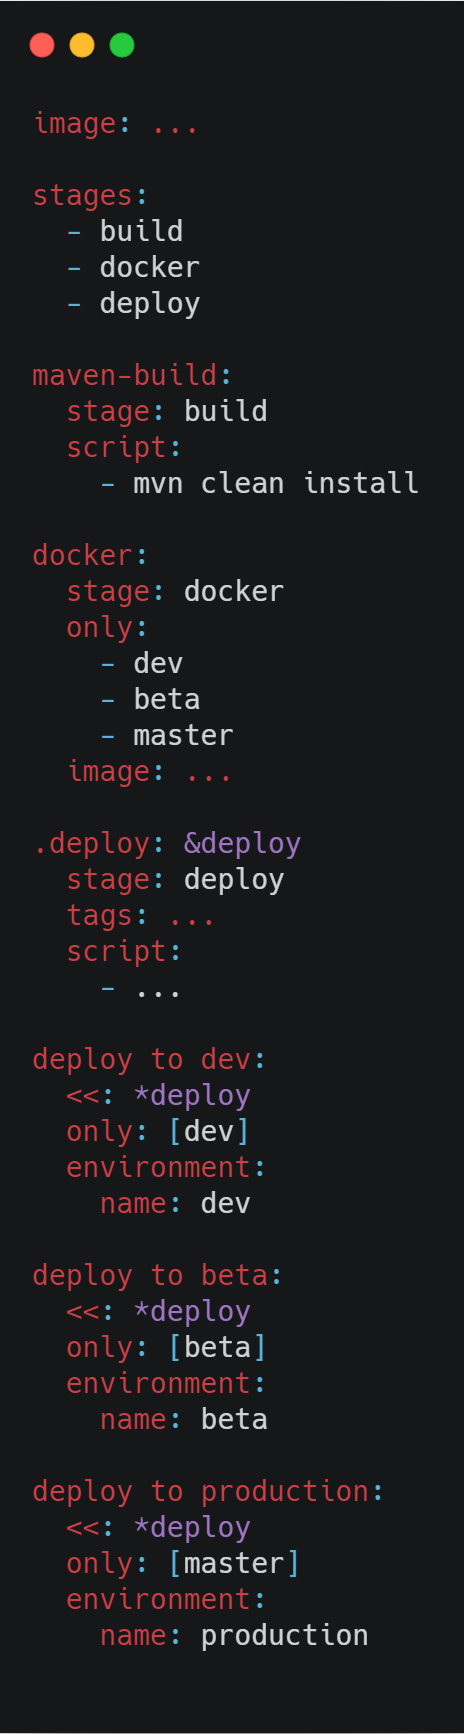
\includegraphics[width=0.35\textwidth]{cicdyaml}  
		\caption{ตัวอย่างไฟล์ .gitlab-ci.yml ในการตั้งค่าให้กับ Gitlab CI/CD}
		\label{Fig:cicdyaml}
	\end{figure}		
\end{enumerate}

\section{รายละเอียดของงานที่ปฏิบัติ}
ในการปฏิบัติงานครั้งนี้ได้ทำการพัฒนาระบบจัดการโฆษณาแบบจำกัดจำนวนการคลิกและการแสดงโฆษณาเฉพาะฟังก์ชันหลักที่จำเป็น เพื่อให้สามารถส่งมอบงานได้เร็วที่สุดและสามารถทำงานได้จริง ได้แก่ ฟังก์ชันการจำกัดการแสดงโฆษณาของร้านด้วยจำนวนการคลิกโฆษณา กับฟังก์ชันการส่งอีเมลรายงานผลการโฆษณากลับไปยังลูกค้าโดยอัตโนมัติทุก ๆ สัปดาห์ 
ระบบจัดการโฆษณาแบบจำกัดจำนวนการคลิกและการแสดงโฆษณาที่พัฒนาขึ้นมานั้น ประกอบด้วยเซอร์วิสต่าง ๆ ได้แก่

\begin{figure}[!h]
	\centering
	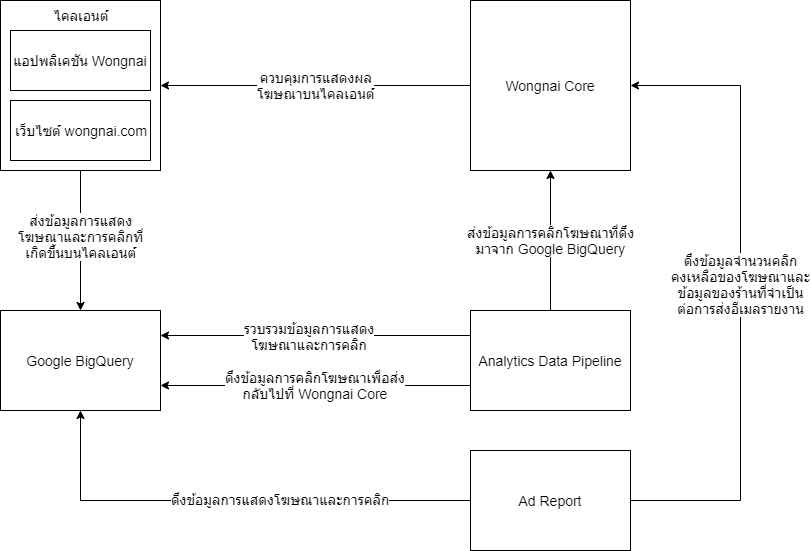
\includegraphics[width=1\textwidth]{ad-report-diagram.png}  
	\caption{แผนผังภาพรวมการทำงานของระบบจัดการโฆษณาแบบจำกัดจำนวนการคลิกและการแสดงโฆษณา}
	\label{Fig:adreport-diagram}
\end{figure}

\begin{enumerate}
	\item Wongnai Core
	
	Wongnai Core เป็นเซอร์วิสหลักของ Wongnai ถูกพัฒนาด้วยภาษา Java ทำหน้าที่ให้บริการหลาย ๆ อย่าง โดยหน้าที่ของ Wongnai Core ที่เกี่ยวข้องกับระบบจัดการโฆษณาแบบจำกัดจำนวนการคลิกและการแสดงโฆษณา ได้แก่ 
	\begin{itemize}
		\item[-] ควบคุมการแสดงผลโฆษณาของเว็บไซต์ wongnai.com และแอปพลิเคชัน Wongnai
		\item[-] รับข้อมูลจำนวนคลิกของโฆษณา เพื่อนำมาอัปเดตในฐานข้อมูลของ Wongnai Core จากนั้นจึงทำการประมวลผลและพิจารณาว่าควรจะนำโฆษณาที่แสดงอยู่ออกหรือไม่ โดยดูจากจำนวนคลิกของโฆษณาว่าเกินกว่าที่จำกัดไว้ตามที่ตกลงกันหรือไม่ ถ้าเกินก็จะหยุดการแสดงโฆษณานั้น ๆ
		\item[-] รอรับการร้องขอข้อมูลจากเซอร์วิส Ad Report เพื่อนำข้อมูลไปใช้ในการสร้างรายงานที่สมบูรณ์ส่งกลับไปยังเจ้าของโฆษณา ซึ่งประกอบไปด้วย ชื่อร้าน, อีเมลของร้าน, จำนวนคลิกโฆษณาของร้านที่ใช้ไปแล้ว และจำนวนคลิกโฆษณาของร้านซื้อไว้
	\end{itemize}
	\item Analytics Data Pipeline
	
	Analytics Data Pipeline เป็นเซอร์วิสขนาดเล็กที่ถูกพัฒนาด้วยภาษา Python ปกติแล้วไคลเอนต์จะส่งข้อมูลเหตุการณ์ต่าง ๆ ที่เกิดขึ้นใน Wongnai มาเก็บใน Google BigQuery ซึ่งข้อมูลเหตุการณ์ต่าง ๆ นั้นมีหลากหลายมาก โดยข้อมูลที่จำเป็นต้องใช้เพื่อให้แสดงโฆษณาแบบจำกัดจำนวนการคลิกได้ ได้แก่ ข้อมูลที่ผู้ใช้ Wongnai ที่คลิกไปยังโฆษณา ซึ่งข้อมูลเหตุการณ์ที่เกิดขึ้นใน Wongnai ทุก ๆ อย่างนั้นจะถูกเก็บอยู่ในตารางข้อมูลเดียวกันทั้งหมด ทำให้ตารางนั้นเป็นตารางที่มีข้อมูลมหาศาล และการดึงข้อมูลจาก Google BigQuery หนึ่งครั้งจะต้องเสียเครดิตตามขนาดของข้อมูลในตาราง หากดึงจากตารางขนาดใหญ่นั้นโดยตรง จะทำให้สูญเสียเครดิตไปโดยไม่จำเป็น Analytics Data Pipeline จึงถูกพัฒนาขึ้นเพื่อแก้ไขปัญหาในจุดนี้ โดยเซอร์วิสนี้จะทำการใช้คำสั่ง SQL เพื่อสร้างตารางข้อมูลใหม่โดยแยกออกมาจากตารางขนาดใหญ่อีกที และรวบรวมข้อมูลเฉพาะส่วนที่ต้องการมาเก็บไว้ ทำให้ได้ตารางข้อมูลที่มีขนาดเล็กลง และมีเฉพาะส่วนที่เราต้องการนำไปใช้จริง ๆ โดยในที่นี้เราจะแยกเฉพาะข้อมูลการแสดงโฆษณาของ Wongnai และข้อมูลที่ผู้ใช้ Wongnai ที่คลิกไปยังโฆษณา หน้าที่อีกอย่างหนึ่งที่สำคัญของเซอร์วิสนี้ คือการนำข้อมูลการคลิกของโฆษณาที่รวมรวบไปเก็บในตารางขนาดเล็กแล้ว ส่งไปอัปเดตที่ฐานข้อมูลของ Wongnai Core ทุก ๆ วัน เพื่อให้ Wongnai Core นำข้อมูลส่วนนี้ไปประมวลผลต่อ

	\item Ad Report
	
	Ad Report เป็นเซอร์วิสใหม่ที่ถูกพัฒนาด้วยภาษา Java ร่วมกับ Spring Boot ทำหน้าที่สร้างอีเมลรายงานสถิติของโฆษณาที่ประกอบไปด้วยข้อมูลต่าง ๆ เช่น จำนวนการแสดงผลโฆษณาต่อวัน, จำนวนผู้ที่คลิกเข้าไปในโฆษณาต่อวัน, จำนวนการคลิกของโฆษณาที่ยังคงเหลือ และจำนวนคลิกของโฆษณาที่ลูกค้าซื้อไว้ เป็นต้น โดยภายในเซอร์วิสนี้ จะมีฟังก์ชันการทำงานหลัก 4 อย่าง ได้แก่
	\begin{itemize}
		\item Statistics Updater
		
		 ฟังก์ชัน Statistics Updater ทำหน้าที่นำข้อมูลของโฆษณาจาก Google BigQuery มาอัปเดตในฐานข้อมูลของ Ad Report กรณีที่ข้อมูลที่เข้ามาเป็นของร้านที่ไม่เคยปรากฏอยู่ในฐานข้อมูลของ Ad Report (เป็นร้านที่ลงโฆษณากับ Wongnai เป็นครั้งแรก) ก็จะทำการเรียกฟังก์ชัน Retrieve Data เพื่อร้องขอข้อมูลจาก Wongnai Core ซึ่งประกอบไปด้วยชื่อร้าน และอีเมลของร้าน นำไปประกอบในการทำรายงานที่สมบูรณ์และส่งอีเมลกลับไปได้
		\item Report
		
		ฟังก์ชัน Report ทำหน้าที่สร้างรายงานที่จะส่งไปพร้อมกับอีเมลให้กับลูกค้า
		\item Report Email
		
		ฟังกชัน Report Email ทำหน้าที่สร้างอีเมลพร้อมกับแนบไฟล์รายงานที่ได้จากฟังก์ชัน Report ส่งไปยังอีเมลของลูกค้า
		\item Retrieve Data
		
		ฟังกชัน Retrieve Data ทำหน้าหน้าที่ร้องขอข้อมูลที่จำเป็นจาก Wongnai Core โดยใช้โปรโตคอล HTTP เพื่อนำไปใช้ในการสร้างรายงานและการส่งอีเมลที่สมบูรณ์
	\end{itemize}
	โดยภายใน Ad Report จะมี Cron ซึ่งเป็นเครื่องมือของ Unix ที่จะทำให้สามารถรัน Command Line หรือ Shell Scripts ตามช่วงเวลาที่เรากำหนดไว้ได้โดยอัตโนมัติ ในที่นี้ได้มีการนำ Cron ไปใช้งาน 2 ส่วน ได้แก่
	\begin{itemize}
		\item Daily Statistics Updater
		
		Daily Statistics Updater จะเรียกใช้งานฟังก์ชัน Statistics Updater ทุก ๆ วัน เพื่ออัปเดตฐานข้อมูลของ Ad Report
		\item Weekly Report Email
		
		Weekly Report Email จะเรียกใช้งานฟังก์ชัน Report และ Report Email เพื่อสร้างรายงานสถิติของโฆษณาและส่งอีเมลกลับไปยังลูกค้าทุก ๆ สัปดาห์ ซึ่งจะส่งให้เฉพาะร้านที่ยังจำนวนคลิกโฆษณาคงเหลืออยู่ โดยดูจากข้อมูลที่ร้องขอมาจากฟังก์ชัน Retrieve Data
	\end{itemize}
\end{enumerate}

เซอร์วิสทั้งหมดที่กล่าวมาข้างต้นจะใช้ Docker สร้างอิมเมจของแต่ละเซอร์วิสสำหรับเซอร์วิส และเซิร์ฟเวอร์ที่รันคอนเทนเนอร์ของอิมเมจของแต่ละเซอร์วิสจะถูกจัดการด้วย Kubernetes ทั้งหมด
\begin{figure}[!h]
	\centering
	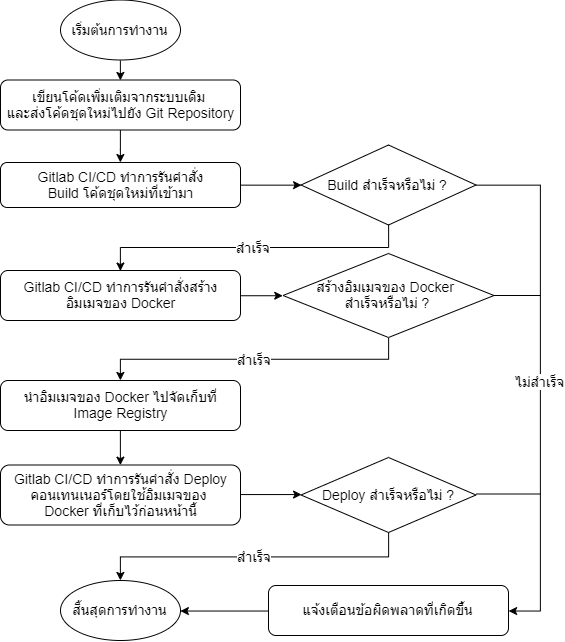
\includegraphics[width=0.9\textwidth]{gitlab-flow.png}  
	\caption{แผนผังวิธีการ Deploy โค้ดชุดใหม่ของเซอร์วิส Ad Report}
	\label{Fig:adreport-diagram}
\end{figure}

สำหรับ Ad Report ซึ่งเป็นเซอร์วิสใหม่นั้น ได้ทำการเพิ่มสคริปสำหรับใช้งาน Gitlab CI/CD เพื่อให้ทำการ Build โค้ด, สร้างอิมเมจ Docker, นำไปจัดเก็บใน Image Registry ที่เป็นพื้นที่สำหรับจัดเก็บอิมเมจ และ Deploy เซอร์วิสโดยอัตโนมัติ การนำอิมเมจ Docker ที่ได้ไป Deploy เป็นคอนเทนเนอร์บนเครื่องเซิร์ฟเวอร์จะมี Project Eastern ซึ่งเป็นไลบรารีที่ช่วย Deploy คอนเทนเนอร์บน Kubernetes และช่วยจัดการ Environment ที่จะ Deploy ให้ ~\cite{eastern} 

\section{ลักษณะขั้นตอนการทำงาน}
ทีม Development ของบริษัท วงใน มีเดีย จำกัด (สำนักงานใหญ่) จะถูกแบ่งออกเป็นทีมย่อย ๆ ตามประเภทของงานที่รับผิดชอบ เรียกว่า Squad ซึ่งจะเป็นทีมแบบ Cross-Functional กล่าวคือ ภายในทีมจะประกอบไปด้วยหลาย ๆ ฝ่าย ได้แก่ Project Manager, UX/UI Designer, Software Engineer (Frontend), Software Engineer (Backend), Software Engineer (iOS), Software Engineer (Android) และ Quality Assurance Engineer โดยแต่ละ Squad อาจจะฝ่ายอื่น ๆ เพิ่มเติมแตกต่างกันไป ขึ้นอยู่กับลักษณะของงานที่รับผิดชอบ โดยแต่ละ Squad นั้นจะทำงานโดยใช้ Scrum Framework เป็นหลัก Scrum จะทำงานเป็นวงรอบ (Sprint) แต่ละรอบนั้นจะเท่ากับ 2 สัปดาห์ ภายใน Sprint จะกิจกรรมที่สำคัญต่าง ๆ ดังต่อไปนี้
\begin{enumerate}
	\item Sprint Planning
	
	เป็นการประชุมตอนต้น Sprint เพื่อรับมอบหมายงานจาก Project Manager และเป็นการประชุมเพื่อปรึกษาหาวิธีการทำงานและวิธีการแก้ไขปัญหาต่าง ๆ ที่เกี่ยวกับงานที่ได้รับมอบหมาย
	
	\item Daily Meeting
	
	เป็นการประชุมแบบสั้น ๆ ประจำวัน มีจุดประสงค์เพื่อให้สมาชิกทีมรับทราบความคืบหน้าของงานที่แต่ละคนกำลังทำอยู่และทราบปัญหาที่เกิดขึ้นระหว่างการทำงาน
	
	\item Backlog Refinement Meeting
	
	ปกติเมื่อ Squad ได้รับมอบหมายให้ทำงานใหม่ ๆ งานนั้นจะถูกจัดไว้ใน Features Backlog ก่อน ซึ่งงานที่อยู่ในนี้จะถูกนำเข้า Sprint ถัด ๆ ไป ขึ้นอยู่กับการตัดสินใจของ Project Manager การประชุมนี้จะจัดตอนกลาง Sprint เพื่อพิจารณางานที่อยู่ Features Backlog ว่าควรจะทำอย่างไร, เป็นงานสำคัญที่ต้องเอามาเท่าก่อนหรือไม่ และประเมินเวลาที่จะต้องใช้ในการทำงานชิ้นนี้ เป็นต้น
	
	\item Retrospective Meeting
	
	เป็นการประชุมตอนปลาย Sprint เพื่อสรุปการทำงานที่ได้ทำไปในรอบ และให้สมาชิกภายในทีมอธิบายปัญหาที่เกิดขึ้นในรอบ รวมไปถึงเรื่องราวดี ๆ ที่เกิดขึ้นในรอบด้วย เพื่อนำไปปรับปรุงการทำงานในรอบถัดไป
\end{enumerate}

การติดต่อสื่อสารภายในองค์กรจะใช้โปรแกรม Slack เป็นหลัก สถานะของงานภายในทีมสามารถดูได้จาก Kanban Board ซึ่งเป็นบอร์ดที่ตั้งอยู่ในพื้นที่ทำงาน และ Asana ซึ่งเป็นระบบออนไลน์ที่จะทำให้สมาชิกภายในทีมสามารถทราบสถานะของงานได้อย่างรวดเร็ว ภายในกระบวนการทำงาน สถานะของงานจะเป็นไปตามดังต่อไปนี้

\begin{enumerate}
	\item To do
	
	งานที่ยังไม่ได้เริ่มทำ แต่อยู่ในรอบแล้วจะมีสถานะเป็น To do
	
	\item In progress
	
	งานที่กำลังทำอยู่จะมีสถานะเป็น In progress
	
	\item Review
	
	เมื่องานที่ทำอยู่เสร็จแล้ว ก่อนที่จะนำงานส่วนที่ทำเข้าไปใน Beta Environment ของเซิฟเวอร์ ซึ่งเป็น Environment ที่มีไว้ทดสอบก่อนที่จะใช้งานจริง โค้ดที่เขียนขึ้นมาจะต้องผ่านการตรวจสอบจาก Software Engineer คนอื่นอย่างน้อย 2 คนก่อน จึงจะสามารถส่งไปให้ Quality Assurance Engineer ทำการทดสอบต่อได้
	
	\item Review passed
	
	เมื่องานที่ทำอยู่ผ่านการตรวจสอบโดย Software Engineer คนอื่นครบ 2 คนแล้ว งานจะอยู่ในสถานะ Review passed 
	
	\item Testing
	งานที่อยู่ในสถานะ Review passed จะถูกส่งต่อให้ Quality Assurance Engineer ทดสอบ ซึ่งก่อนที่จะให้ Quality Assurance Engineer ทดสอบนั้น จะต้องเตรียมวิธีการทดสอบและเตรียมข้อมูลให้เรียบร้อยก่อน
	
	\item Test passed
	
	เมื่อ Quality Assurance Engineer ทดสอบเสร็จแล้ว งานจะอยู่ในสถานะ Test passed สามารถนำงานเข้า Beta Environment ได้เลย
	
	\item Done
	
	เมื่อนำงานเข้าไปใน Beta Environment เสร็จแล้ว งานจะมีสถานะเป็น Done แต่อย่างไรก็ตาม เจ้าของงานจะต้องติดตามงานของตัวเองจนกว่างานจะขึ้นอยู่บนระบบที่ใช้งานจริง (Production Environment)
\end{enumerate}

โดยส่วนมากแล้ว ถ้าเป็นงานที่เป็นการเขียนโค้ดจะมีกระบวนการทำงานตามที่กล่าวมาข้างต้น แต่อย่างไรก็ตามงานบางชนิดไม่จำเป็นต้องทำตามกระบวนการอย่างเคร่งครัดก็ได้ ขึ้นอยู่กับความเหมาะสมของงานว่าควรจะเป็นแบบไหน และในการทำงานของทีม Development ที่เป็นการเขียนโค้ดจะใช้ Test Driven Development (TDD) เป็นหลัก เป็นการเขียนชุดทดสอบของโค้ดขึ้นมาก่อน แล้วรันชุดทดสอบให้เกิดข้อผิดพลาด จากนั้นจึงเขียนโค้ดเพื่อแก้ไขข้อผิดพลาดนั้น ระหว่างการเขียนโค้ดจะต้องคอยคำนึงถึงคุณภาพของโค้ด หากมีโค้ดส่วนที่ไม่จำเป็นกจะต้องทำการ Refactor โค้ดส่วนนั้นด้วย โดยการ Refactor จะเป็นการลบโค้ดส่วนที่ไม่จำเป็นออก และนำโค้ดส่วนอื่น ๆ มาใช้ซ้ำให้มากที่สุด เพื่อให้โค้ดสั้นลง, มีคุณภาพ และ Software Engineer คนอื่น สามารถพัฒนาโค้ดส่วนนี้ต่อได้ง่าย

\begin{figure}[!h]
	\centering
	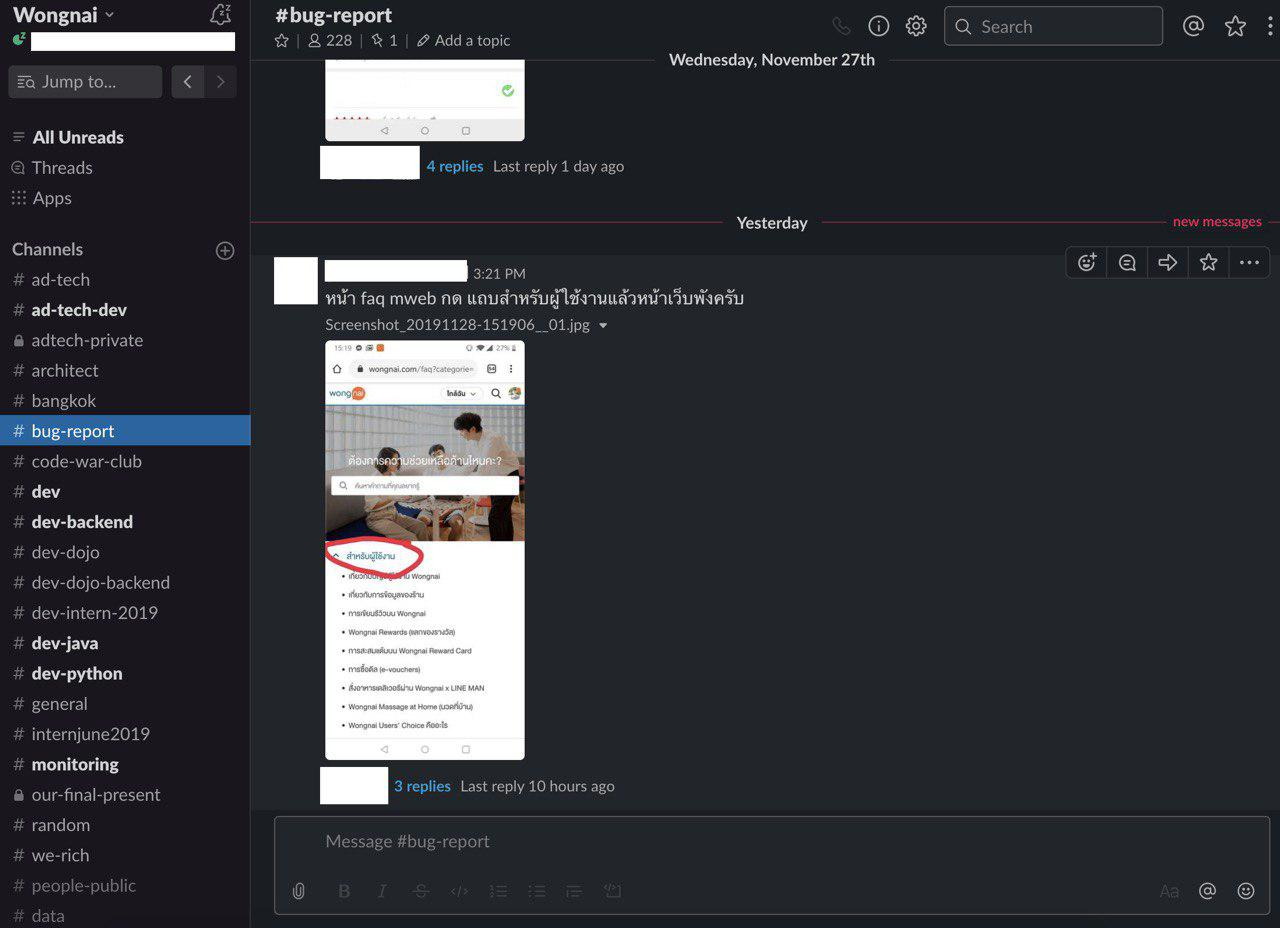
\includegraphics[width=1\textwidth]{slack}  
	\caption{ตัวอย่างของโปรแกรม Slack}
	\label{Fig:slack}
\end{figure}

\begin{figure}[!h]
	\centering
	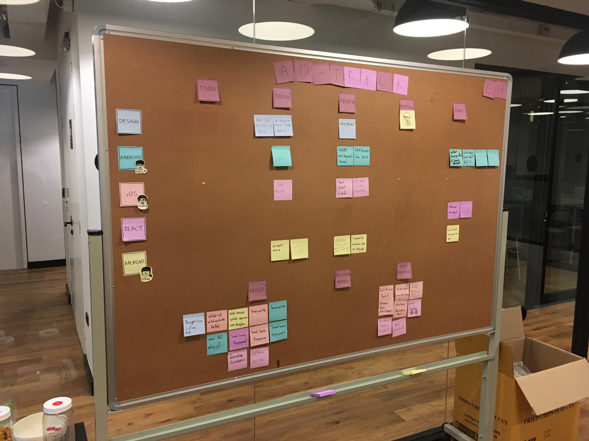
\includegraphics[width=1\textwidth]{kanban-board.png}  
	\caption{Kanban Board ที่ตั้งอยู่ในพื้นที่ทำงาน}
	\label{Fig:kanban-board}
\end{figure}